The results visualization system provides a graphical summary of the progression of an optimziation. It was written using Ruby On Rails and takes advantage of two graphical plotting tools: gcharts and graphviz. Gcharts is used to generate the graphcial plots of relevant optimization metrics from different optimizations. The graphviz package is used to render images of the 

\subsection{Optimization Metrics}
The progress of the optimziation is charachertized on a per generation bassis. Relevant metrics include: 
\begin{itemize}
	\item Average fitness
	\item Maximum fitness
\end{itemize}

For a good optimization one would expect both the maximum fitness and the average fitness to increase from one generation to the next. However, the data represnetation provides valuable information regarding the relative values of the maximum and the average fitness. If the average fitness begins to approach a value close to the maximum fitness, this is an indication that the population is becoming too homogeneous and it is unreasonable to expect further optimization to result in large fitness gains.
\begin{figure}[!hbp]
  \centering
  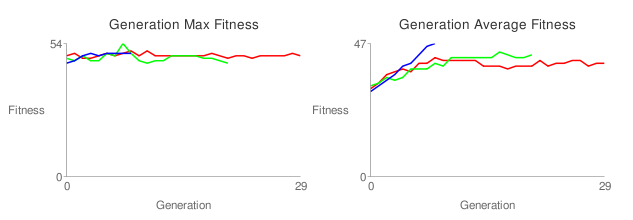
\includegraphics[width = .75\textwidth]{images/sample_graphs}
  \caption{Example metric graphs for maximum and average fitness. \label{fig:sample_graphs}}
\end{figure}
Since the optimization was sub-devided into three separate optimization runs to test the three different fitness testing methods, the visualization tool also provides graphical representation of each of the three sub-data sets simultaneously. This representation allows a quick comparison between the effectiveness of the three different fitness evaluation methods.  

\subsection{TM Representation}
The vizualization of individual TMs provides a valuable tool for their inspection. There are litterally thousands of TMs created over the course of an optimziation, and graphviz package allows or the creation of a state transition diagram for quick visual inspection of particular TMs. Figure \ref{fig:example_TM} is the state transition diagram for the example TM in Table \ref{tab:example_TM}. This visual representation is much easier to interperate than the state transition table. 

\begin{figure}[!hbp]
	\centering 
	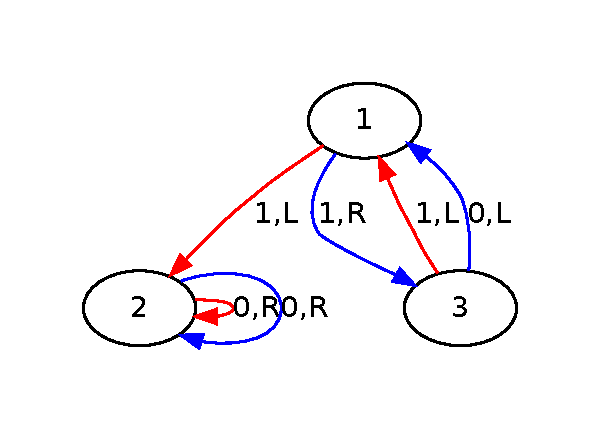
\includegraphics[width=.8\textwidth]{images/example_TM}
	\caption{State transition diagram for notional 3-state TM. Edge color indicates the bit being read from the tape (red=0,blue=1). Edge label indicates the write bit and movement direction for a given transition.}
	\label{fig:example_TM}
\end{figure}
